% --------------------------------------------------------------
% This is all preamble stuff that you don't have to worry about.
% Head down to where it says "Start here" % --------------------------------------------------------------
 
\documentclass[12pt]{article}

\usepackage{listings}
\usepackage[margin=1in]{geometry} 
\usepackage{amsmath,amsthm,amssymb}
\usepackage{graphicx}
\usepackage{hyperref}
\graphicspath{ {../media/} } 

\newcommand{\N}{\mathbb{N}}
\newcommand{\Z}{\mathbb{Z}}
\newcommand\indep{\protect\mathpalette{\protect\independenT}{\perp}}
\def\independenT#1#2{\mathrel{\rlap{$#1#2$}\mkern2mu{#1#2}}}

\newenvironment{theorem}[2][Theorem]{\begin{trivlist}
\item[\hskip \labelsep {\bfseries #1}\hskip \labelsep {\bfseries #2.}]}{\end{trivlist}}
\newenvironment{lemma}[2][Lemma]{\begin{trivlist}
\item[\hskip \labelsep {\bfseries #1}\hskip \labelsep {\bfseries #2.}]}{\end{trivlist}}
\newenvironment{exercise}[2][Exercise]{\begin{trivlist}
\item[\hskip \labelsep {\bfseries #1}\hskip \labelsep {\bfseries #2.}]}{\end{trivlist}}
\newenvironment{reflection}[2][Reflection]{\begin{trivlist}
\item[\hskip \labelsep {\bfseries #1}\hskip \labelsep {\bfseries #2.}]}{\end{trivlist}}
\newenvironment{proposition}[2][Proposition]{\begin{trivlist}
\item[\hskip \labelsep {\bfseries #1}\hskip \labelsep {\bfseries #2.}]}{\end{trivlist}}
\newenvironment{corollary}[2][Corollary]{\begin{trivlist}
\item[\hskip \labelsep {\bfseries #1}\hskip \labelsep {\bfseries #2.}]}{\end{trivlist}}
 
\begin{document}
 
% --------------------------------------------------------------
%                         Start here
% --------------------------------------------------------------
 
%\renewcommand{\qedsymbol}{\filledbox}
 
\title{Assignment 1\\
Big Data Analytics Programming} %if necessary, replace with your course title
\author{Evangelos Ntavelis\\ %replace with your name
r0692337 \\
evangelos.ntavelis@student.kuleuven.be}
 
\maketitle

\tableofcontents

\section{Blocked Matrix Multiplication}

The goal of the first part of the assignment is to test if we can achieve better performance by multiplying two matrices in a blocked fashion rather than following the naive approach. 

Firstly, the implementation of blocked matrix multiplication was something trivial given we had the code of naive method. We had just to make sure that our changes didn't cause any segmentation faults by going over the matrices' limits and how to correctly allocate enormous chunks of memory. We also made sure that the blocked method produced the same results as the naive method.

The more challenging part was to gauge the performance of the algorithm based on different block sizes and inputs. One question is that we should answer if different block sizes perform better depending on how big the input matrices are. Thus, we created different random input matrices whose size was growing exponentially to the factor of 2. For these inputs we tested exponentially growing block-sizes. As the time needed for the program to run grew according to the size of the inputs, we initially planned to present the results in a logarithmic scale graph, but that decreased the readability of the graph.

%\lstinputlisting[language=Python]{./MatrixMultiplication/matrixgen.py}

As we can see in \ref{Figure 1}, the naive method is readily outperformed after increasing the size just a bit. In our last multiplication test, i.e. $4085 \times 4086$ we observe the blocked-8 to perform better than the other block configurations.

\begin{figure}[h]
    \centering
    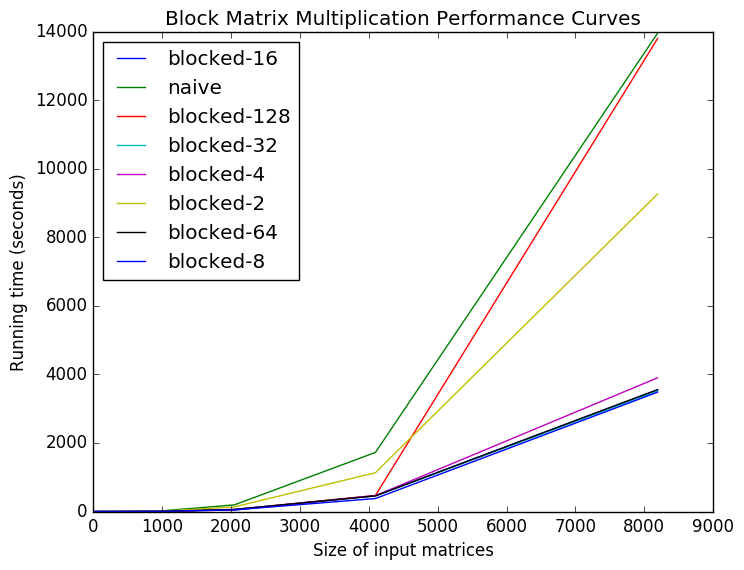
\includegraphics[scale=.8]{graphnew}
    \caption{Running time in seconds - Size of the Matrix}
    \label{Figure 1}
\end{figure}

\section{Spam Filter}

\subsection{Implementing the algorithms}


\subsection{Evaluation Metrics}

For this assignment we used the following set of evaluation metrics: Accuracy, Precision, True Positive Rate (Recall), True Negative Rate (Specificity). We should note that because of the nature of our problem it is more important to have spam e-mail predicted as ham than the other way around. It's better to get emails from both your dream job and a Nigerian prince than getting none!

\begin{enumerate}
  \item \textbf{Accuracy} is the number of correct predictions divided by the total number of predictions made. While accuracy is a good indicator of the robustness of our model there are cases that we encounter the \textit{accuracy paradox}. Accuracy can be misleading when we have classes that differ a lot in size and the model predicts correctly only the label of the bigger(majority) class. The resulting value of the metric would not be representative of the model's predictive power. In our case, the classes have different sizes and thus, we have to complement our evaluation with additional metrics.

    \[ Accuracy = \frac{TP + TN}{TP + FP + TN + FN} \]

  \item \textbf{Precision}, alternatively positive predictive value, and in our context represents the proportion of the emails that are actually spam out of the all the mails we classified as spam. This is a very important metric for us, because as its value approaches 1 the number of misclassified spam emails drops to zero.

    \[ Precision = \frac{TP}{TP + FP} \]

  \item \textbf{True Positive Rate}, or recall, is the number of e-mails which are classified as spam out of all spam mails. In fact, recall shows how effective is our spam filter to block incoming spam e-mails.

    \[ tpRate = \frac{TP}{TP + FN} \]

  \item \textbf{True Negative Rate}, or specificity, on the other hand is the number of e-mails that are classified as ham out of all ham mails. This is the least important metric for us. While optimally we don't want to classify spam mail as ham, this is secondary compared to the other way around.

    \[ tnRate = \frac{TN}{TN + FP} \]

  \item \textbf{F-score}, having produced the precision and recall values of our models we can compute their F-score. Hereby, we compute the balanced F-score (F1-score) as the harmonic mean of the aforementioned metrics. F1 is important as it shows us a combined value of Precision and Recall which are both important in the evaluation of our models.

    \[F1 = 2 \times \frac{precision * recall}{precision + recall}\]


\end{enumerate}


\subsection{Experiments}

\subsubsection{Setting up the experiments}
      The goal of our experimental setup is to be able to find out which parameters affect the performance of our models and in which ways. To do so, we are following an exploratory data analysis approach where, after our initial implementation of the algorithms, we tested them against different combinations of the parameters. 

This approach resulted in an abundance of metrics results to analyze, but also was very challenging. In order to create more than 6.000 experiment settings, while each one of them took from six minutes to half an hour we used a bash script which connected to multiply machines at once and run the experiments. Firstly, there were a lot of experiment that were running simultaneously to a single machine, but for some reason the produced metric timeseries were distorted. We attributed this to the inner mechanisms of the used language, and didn't bother that much.
       
The resulted outputs were then loaded to a Python Notebook and were analysed with the help of the Pandas Framework.

\subsubsection{Naive Bayes Feature Hashing}

\begin{figure}[h]
    \centering
    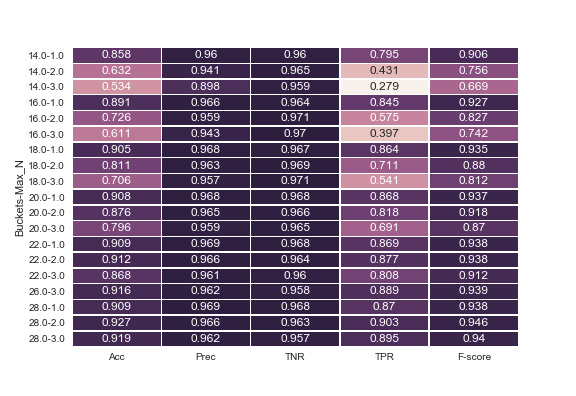
\includegraphics[scale=0.8]{./SpamFilter/code/nbfh}
    \caption{Naive Bayes Feature Hashing - Heatmap}
    \label{nbfh}
\end{figure}



Observations:
    
\begin{itemize}
          
      \item \textit{Increasing the N-grams decreases the metrics values. }
          This is probably due to the noise we create by all the combinations we introduce to our vocabulary. All this noise creates collisions.

        \item \textit{More buckets let us achieve high accuracy even with higher n-grams.}
          We have enough space to reduce the collisions created by the aforementioned noise.

      \item \textit{For smaller bucket sizes, 1-grams provide the best solution.} As we increase the buckets number we get the best overall metrics for 2-grams.
          Combinations of two words provide insight on whether the e-mail is spam/ham without creating noise. Yet the vocabulary increases a lot from the 1-gram and we need more space to accommodate it.

        \item \textit{Threshold changes affect our metrics only when put on extreme values.}
          This is due to the nature of Naive Bayes model, which pushes the probabilities near 0 and 1.

        \item \textit{As we increase the buckets number we observe a saturation of the improvement of our model.}
          Also to be expected, as from one point onwards collisions stop to be a problem and we only create a sparse array.

     \end{itemize}

\begin{figure}[h]
    \centering
    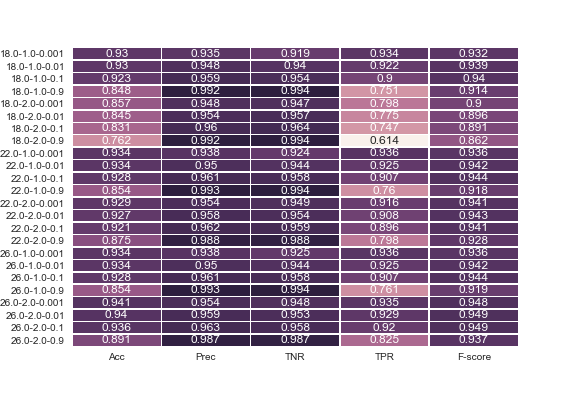
\includegraphics[scale=0.8]{./SpamFilter/code/nbfhthres}
    \caption{Naive Bayes Feature Hashing - Threshold - Heatmap}
    \label{nbfht}
\end{figure}

\begin{figure}[h]
    \centering
    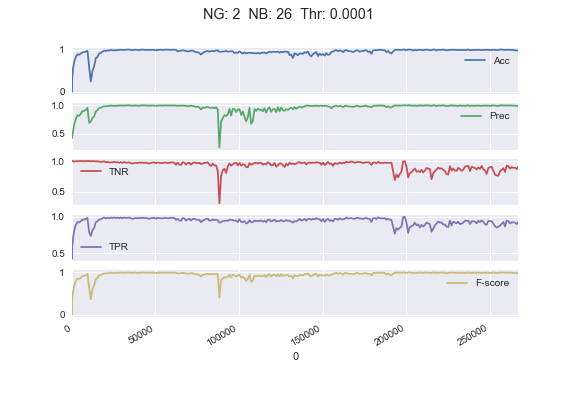
\includegraphics[scale=0.8]{./SpamFilter/code/nbfhcurve}
    \caption{Naive Bayes Feature Hashing - Evaluation Metrics}
    \label{nbfhc}
\end{figure}



Scalability:
    
     In order to determine how scalable each configuration is, we don't have to run the experiments against the whole dataset. The memory requirements are constant and as it is online learning the time performance can be measured single mail-wise. Thus, by measuring the performance against the small dataset of 1000 mails we have enough samples to overcome the randomness of a single case. 
   
      



\subsubsection{Naive Bayes Count-Min-Sketch}

Observations:

\begin{figure}[h]
    \centering
    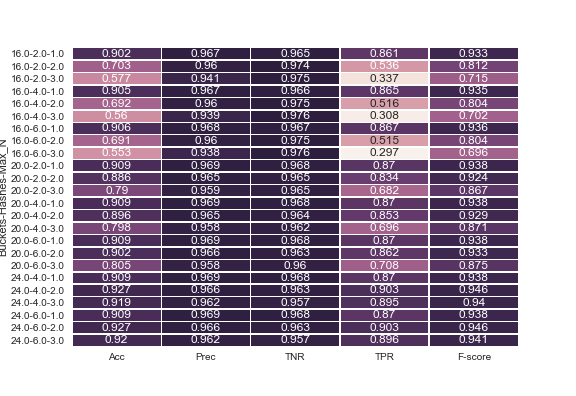
\includegraphics[scale=0.8]{./SpamFilter/code/nbcms}
    \caption{Naive Bayes Count-Min-Sketch - Heatmap}
    \label{nbcms}
\end{figure}


\begin{figure}[h]
    \centering
    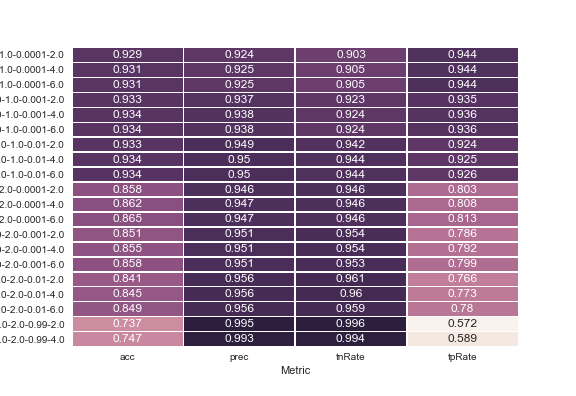
\includegraphics[scale=0.8]{./SpamFilter/code/nbcmsthres}
    \caption{Naive Bayes Count-Min-Sketch - Threshold - Heatmap}
    \label{nbcmst}
\end{figure}


\begin{figure}[h]
    \centering
    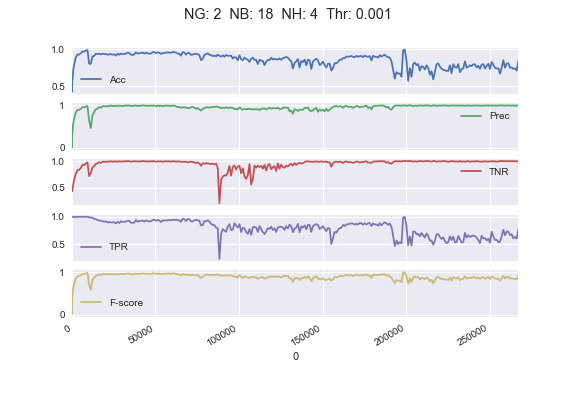
\includegraphics[scale=0.8]{./SpamFilter/code/nbcmscurve}
    \caption{Naive Bayes Count-Min-Sketch - Evaluation Metrics} 
    \label{nbcmsc}
\end{figure}


\begin{itemize}
      \item 
        \textit{The observations made for the Feature Hashing algorithm also stand here.}

        \item
        \textit{The larger the number of buckets the lesser the effect of adding more hashing functions}

        \item
          \textit{We can achieve the same metric values as Feature Hashing for smaller bucket sizes} This become more evident as the bucket number increases. For instance for NBCMS with 4 hash functions and $2^{24}$ buckets we observe the same average performance for an $2^{28}$ NBFH model, only by using $1/4$ of the space. 


\end{itemize}

\subsubsection{Perceptron Feature Hashing}

\begin{figure}[h]
    \centering
    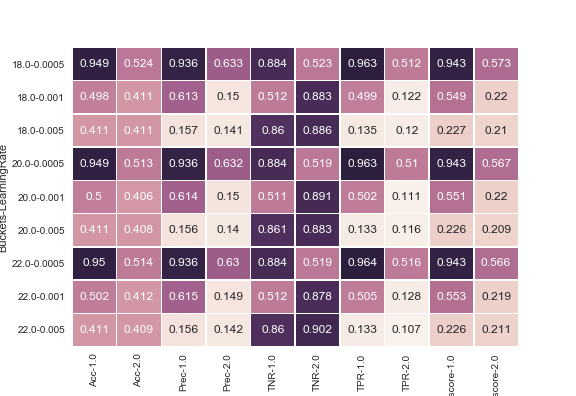
\includegraphics[scale=0.8]{./SpamFilter/code/pfh}
    \caption{Perceptron Feature Hashing - Heatmap}
    \label{pfhhm}
\end{figure}

\begin{figure}[h]
    \centering
    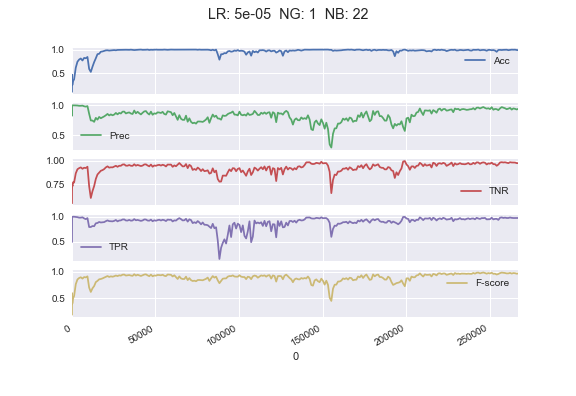
\includegraphics[scale=0.8]{./SpamFilter/code/pfhcurve}
    \caption{Perceptron Feature Hashing - Evaluation Metrics}
    \label{pfhc}
\end{figure}


Observations: 
\begin{itemize}
        \item
          \textit{We have out best results for n-gram = 1}.

        \item
          \textit{The smaller the number of buckets, the smaller the learning rate that achieves best performance.}
          We should attribute this to the fact that by using less buckets, each weight represents more words, so each iteration ends up altering our  table a lot. This shifts as we increase the size of the table and decrease the number of collisions. Thus, by allowing individual weights to adapt more readily our model learns better. The cap is at 0.0005 of learning step where we achieve our best performance.




\end{itemize}

\subsubsection{Perceptron Count-Median-Sketch}
    
    We observed the same differences that Naive Bayes Count-Min-Sketch had with Naive Bayes Feature Hashing. 

\begin{figure}[h]
    \centering
    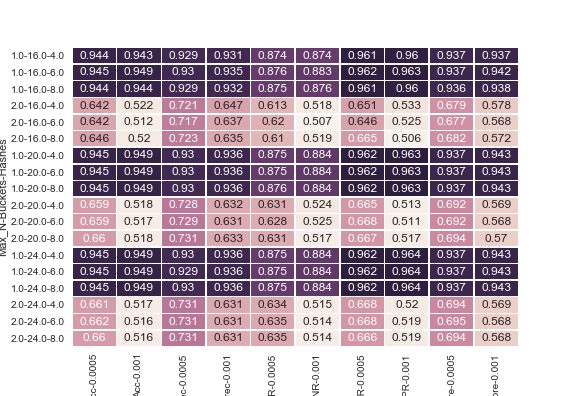
\includegraphics[scale=0.8]{./SpamFilter/code/pcms}
    \caption{Perceptron Count-Median-Sketch - Heatmap}
    \label{pcms}
\end{figure}

\begin{figure}[h]
    \centering
    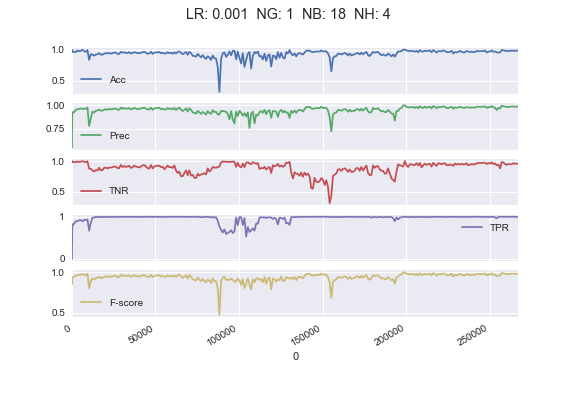
\includegraphics[scale=0.8]{./SpamFilter/code/pcmscurve}
    \caption{Perceptron Count-Median-Sketch - Evaluation Metrics}
    \label{pcmsc}
\end{figure}

\subsubsection{General Remarks}

We observed that our Perceptron performed better than the Naive Bayes in accuracy but it was vice versa in F1-score.Also, to achieve for its best result it needed less buckets, although we have to mention that the perceptron uses double for its weights which uses the same bytes as the two tables of integers the NB uses. 

In both cases the Count-Min-Sketch permitted us to achieve same performance while minimizing the space requirements. 

In order to pick our best model, we chose the configuration that achieved both good accuracy and f1-score, with the later being more important. We only paid attention to the first three decimal points of our metrics, which resulted for many different configurations to bear similar results. From this set we picked the one which also minimized the time and space requirements of our algorithm.

On the next list we can see the detailed results of the parameters we used to achieve the best performance for each of our models.
 

\begin{itemize}
 \item NBFH, acc: 9.4, f1: 9.49\\ 
 \item NBCMS, acc:  9.39, f1:  9.49\\ 
 \item PFH, acc: 9.5, f1: 9.43\\ 
 \item  PCMS, acc: 9.49, f1: 9.43\\ 
\end{itemize}


%
%\begin{center}
%  \begin{tabular}{ |c||c|c|c|c||c|c|} } 
%  \hline
% Model & Buckets(log) & Thres/L.Rate & Hashes & N-grams & Av.Acc & Av.F1-score \\ 
% \hline
% NBFH & 26 & 0.01 & - & 2 & 9.4 & 9.49\\ 
% NBCMS & 26 & 0.01 & 4 & 2 & 9.4 & 9.49\\ 
% PFH & 22 & 0.0005 & - & 1 & 9.5 & 9.43\\ 
% PCMS & 18 & 0.001 & 4 & 2 & 9.49 & 9.43\\ 
% \hline
%\end{tabular}
%\end{center}




\section{Personal Remarks}

I had a suboptimal approach this assignment, I focused on creating a huge dataset of possible configurations of the models parameters. It was a tedious task that I ended up spending an enormous amount of time on trying to run all those experiments, debug and reconfigure the automation of this task, parse the abundant results and visualize them. I learned a ton through the process, both in technical stuff (Pandas, Bash, Unix, Data Manipulation and Visualisation, Python) and meta-knowledge things as that ad-hoc programming is a bad bad thing that gonna haunt you for the days to come. Given this through, in the end I didn't have any time left to focus on the optimization of the implementation of the methods themselves. 

\section{Resources}

\begin{itemize}

  \item \hyperlink{https://en.wikipedia.org/wiki/Evaluation_of_binary_classifiersx}{Wikipedia: Evaluation of binary classifiers}
  \item https://machinelearningmastery.com/classification-accuracy-is-not-enough-more-performance-measures-you-can-use/
  \item https://tryolabs.com/blog/2013/03/25/why-accuracy-alone-bad-measure-classification-tasks-and-what-we-can-do-about-it/
  \item Machine Learning and Inductive Inference Lecture Notes

\end{itemize}

\end{document}
